%!TEX root=../document.tex

\section{Ergebnisse}
\subsection{Aufgabe a}
Der erste Schritt war es in \verb|stm32f3xx_it.c| den \verb|EXTI0_IRQHander| zu implementieren:

\begin{lstlisting}[language=C]
void EXTI0_IRQHandler(void){
	HAL_GPIO_EXTI_IRQHandler(GPIO_PIN_0);
}	
\end{lstlisting}

Weiters wurde eine Funktion erstellt, welche den Port bzw. den Pin für den User-Button initialisiert. Zusätzlich werden für den Interrupt, welcher beim Drücken des Userbuttons ausgelöst wird, auf die Priorität 2 gesetzt:

\begin{lstlisting}[language=C]
void BUTTON_Init(void){
	__HAL_RCC_GPIOA_CLK_ENABLE();
	GPIO_InitStruct.Pin = GPIO_PIN_0;
	GPIO_InitStruct.Mode = GPIO_MODE_IT_RISING;
	GPIO_InitStruct.Pull = GPIO_NOPULL;
	GPIO_InitStruct.Speed = GPIO_SPEED_FREQ_HIGH;
	HAL_GPIO_Init(GPIOA, &GPIO_InitStruct);
	HAL_NVIC_SetPriority(EXTI0_IRQn,2,0);
	HAL_NVIC_EnableIRQ(EXTI0_IRQn);
}
\end{lstlisting}

Danach wurde die Funktion \verb|HAL_GPIO_EXTI_Callback| implementiert. Dieser Callback wird jedesmal aufgerufen, sobald der Userbutton gedrückt wird:

\begin{lstlisting}[language=C]
void HAL_GPIO_EXTI_Callback(uint16_t GPIO_PIN){
BSP_LED_Toggle(LED_RED);
}
\end{lstlisting}

Der nächste Schritt ist es nun 2 LEDs zum Blinken zu bringen. Eine davon soll mit \verb|HAL_Delay| in der main Funktion blinkend gemacht werden, die andere soll auf den \verb|SYSTICK_Callback| reagieren und somit die andere LED zum blinken zu bringen. Der \verb|SYSTICK_Callback| wird automatisch jede Millisekunde aufgerufen, und es ermöglicht es somit Sachen \glqq Parallel\grqq\ zur main Methode auszuführen. Daher im \verb|SYSTICK_Callback| nicht gewartet werden kann, muss ein globaler Counter angesetzt werden, welcher bei jedem Aufruf des Callbacks, d.h. jede Sekunde, den Counter hochzählt.

\begin{lstlisting}[language=C]
void HAL_SYSTICK_Callback(void) {
	counter++;
	// Jede 250ms die LED togglen
	if (counter % 250 == 0) {
		BSP_LED_Toggle(LED_ORANGE);
	}
}
\end{lstlisting}

In der main Methode wurden zuerst die benötigten Init Methoden ausgeführt, und danach in einer While-True Schleife alle 500ms eine LED getoggled:

\begin{lstlisting}[language=C]
int main(void) {
	HAL_Init();
	BUTTON_Init();
	BSP_LED_Init(LED_BLUE);
	BSP_LED_Init(LED_RED);
	BSP_LED_Init(LED_ORANGE);
	
	for(;;){
		HAL_Delay(500);
		BSP_LED_Toggle(LED_BLUE);
	}
}
\end{lstlisting}
\subsection{Aufgabe B}
Bei dieser Aufgabe soll beim Betätigen der Taste in eine Interruptroutine gewechselt werden, in welcher eine LED blinkt. Während dieser Routine steht alles still, außer der Systick-Interrupt. Um zu gewährleisten dass dieser auch funktioniert während der Interruptroutine des Buttons, muss diesem eine höhere Priorität als dem EXTI0 Interrupt gegeben werden:

\begin{lstlisting}[language=C]
int main(void) {
	HAL_Init();
	// Systick interrupt prioritaet hoeher als die vom Button
	HAL_NVIC_SetPriority(SysTick_IRQn,0,0);
	HAL_NVIC_SetPriority(EXTI0_IRQn,1,0);
	HAL_NVIC_EnableIRQ(EXTI0_IRQn);
	
	
	BUTTON_Init();
	BSP_LED_Init(LED_BLUE);
	BSP_LED_Init(LED_RED);
	BSP_LED_Init(LED_ORANGE);
	
	for(;;){
		HAL_Delay(500);
		BSP_LED_Toggle(LED_BLUE);
	}
}
\end{lstlisting}

Der Callback des Buttons wurde folgendermaßen definiert:

\begin{lstlisting}[language=C]
void HAL_GPIO_EXTI_Callback(uint16_t GPIO_PIN){
	int i;
	for(i = 0; i < 20; i++){
		BSP_LED_Toggle(LED_RED);
		HAL_Delay(250);
	}
}
\end{lstlisting}

Falls der Systick Interrupt \textbf{NICHT} höhere Priorität als der EXTI0 Interrupt hätte, würde in der Interruptroutine des Buttons festgehangen blieben werden, daher \verb|HAL_Delay| intern Systick abfragt um die gewartete Zeit zu bestimmen.

\clearpage
\subsection{Aufgabe C}
Bei dieser Aufgabe geht es darum, seinen eigenen Interrupt zu definieren. Der erste Schritt ist es im File \verb|startup/startup_stm32f303xc.s| seinen eigenen Interrupt in der Tabelle zu definieren. Hierbei muss man darauf achten, seinen eigenen Interrupt in einem freien Slot zu definieren. Ich habe meinen Interrupt in der Zeile 232 nach dem \verb|COMP7_IRQHandler| definiert:

\begin{minipage}{\linewidth}
	\centering
	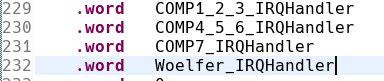
\includegraphics[width=0.8\linewidth]{images/1}
	\figcaption{Woelfer\_IRQHandler wurde definiert}
\end{minipage}

Jeder Interrupt hat eine gewisse Nummer, diese sind im File \verb|CMSIS/device/stm32f303xc.h| einzusehen. Relevant hierbei ist die Nummer von jenem Interrupt, nach welchem mein Interrupt definiert wurde, also \verb|COMP7|:

\begin{minipage}{\linewidth}
	\centering
	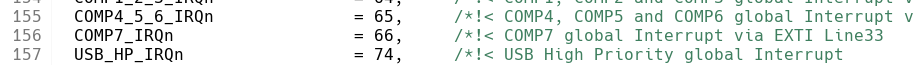
\includegraphics[width=0.8\linewidth]{images/2}
	\figcaption{Interrupt Nummer des COMP7 Interrupts}
\end{minipage}

Nun muss der selbstdefinierte Interrupt diese Nummer plus 1 besitzen:

\begin{lstlisting}[language=C]
#define Woelfer_IRQn (COMP7_IRQn+1)
\end{lstlisting}

Nun muss der Interrupt mit der beschrieben Nummer initialisiert werden:

\begin{lstlisting}[language=C]
HAL_NVIC_EnableIRQ(Woelfer_IRQn);
\end{lstlisting}

Der nächste Schritt ist jene Funktion zu implementieren, welche aufgerufen wird sobald der Interrupt gefeuert wird:

\begin{lstlisting}[language=C]
void Woelfer_IRQHandler(void){
	BSP_LED_Toggle(LED_GREEN);
}
\end{lstlisting}

Der letzte Schritt ist den Interrupt auszulösen, dieser soll ausgelöst werden sobald auf den Userbutton gedrückt wird:

\begin{lstlisting}[language=C]
void HAL_GPIO_EXTI_Callback(uint16_t GPIO_PIN){
	BSP_LED_Toggle(LED_RED);
	HAL_NVIC_SetPendingIRQ(Woelfer_IRQn);
}
\end{lstlisting}
